\documentclass[10pt]{article}
\usepackage{xr}

\usepackage{graphicx}
\usepackage{amsfonts}
\usepackage{pifont}
\newcommand{\cmark}{\ding{51}}%
\newcommand{\xmark}{\ding{55}}%

\linespread{1}
\addtolength{\oddsidemargin}{-2.5cm}
%\addtolength{\evensidemargin}{-3cm}
\addtolength{\textwidth}{2.5cm}

\setcounter{figure}{1}    
\begin{document}




\begin{figure}
\caption{Power verse false discovery rates for Eagle and the multiple-locus methods. Plots for only those simulation 
scenarios where all multiple-locus methods could be implemented are shown.  Eagle has the highest power across the four 
scenarios but MLMM also performs well. }
\label{figpowermultiple}
\begin{center}
\includegraphics[width=15cm, height=15cm]{power1main.eps}
\end{center}

\end{figure}






\end{document}
